\documentclass{beamer}
\usecolortheme{whale}
\usecolortheme{orchid}
\useinnertheme[shadow=false]{rounded}
\useoutertheme[footline=authortitle]{miniframes}

\usepackage{multimedia}

\usepackage[french]{babel}

\usepackage[utf8]{inputenc}
\usepackage[T1]{fontenc}

\usepackage{multimedia}
\usepackage{amssymb}
\usepackage{amsmath}

\title[CAP 2016]
{Optimisation quadratique pour l'apprentissage en ligne d'un bandit contextuel} 
%\subtitle{Day 1 : Encoding and signal processing with neural assemblies : definitions, models, simulations, experiments}

\author{Hongliang Zhong$^1$ et Emmanuel Daucé$^2$}

\institute{1. Aix Marseille Univ, CNRS, Centrale Marseille, LIF, Laboratoire d'Informatique Fondamentale, Marseille, France \\
2. Aix Marseille Univ, Inserm, INS, Institut de Neurosciences des Systèmes, Marseille, France}

\date{5 Juillet 2014}

\begin{document}

\begin{frame}\titlepage
\end{frame}

\begin{frame}\frametitle{Aprentissage en ligne}
%Processus d'apprentissage pour lequel se répètent les opérations suivantes~:
Une organisation séquentielle de l'apprentissage~:
\begin{exampleblock}{}
Pour tout $t \in 1,... T$~:
\begin{enumerate}
	\item Lire  le vecteur d'observation $x_t \in \mathbb{R}^d$
	\item Choisir une réponse (étiquette) $\tilde{y}_t \in \{1,...,K\}$ %selon $\Pi_{t-1}$ (politique).
	\item Lire l'information (feedback) $f_t$
	\item Mettre à jour le classifieur $W_t$
\end{enumerate}
\end{exampleblock}

Problèmes en lien avec ce formalisme :
\begin{itemize}
	\item Bandits contextuels \cite{lai1985asymptotically,auer2002finite}
	\item Apprentissage en ligne supervisé \cite{rosenblatt1958perceptron,duda1973pattern}
\end{itemize}

\end{frame}

\begin{frame}\frametitle{Univers actionnables (Bandit problem)}
	\begin{itemize}
		\item Exemple des machines à sous : répertoire d'actions
		\item Apprentissage actif : 
		\begin{itemize}
			\item Apprendre les conséquences
			\item L'univers est sondé à travers des actions
			\item Approche séquentielle par essais/erreurs
		\end{itemize}
		\item Chaque action $y$ apporte:
		\begin{itemize}
			\item une gratification (gain) $g$
			\item qui constitue une \textit{information} permettant de mettre à jour un \textit{modèle} $E(g|y)$
		\end{itemize}
		\item Dilemme exploration/exploitation
		\item Notion de regret :
		$$ \sum_{t \in 1,..,T} g^*_t - g_t$$ 
	\end{itemize}
\end{frame}

\begin{frame}
	\frametitle{Classifieurs linéaires}
	\begin{itemize}
		\item Tâche : identifier des caractère, des visages, des objets ...
		\item Observation / espace des observations : $x \in \mathbb{R}^d $ 
		\item Étiquettes : $1,...,K$
		\item Hypothèse : 
		\begin{itemize}
			\item Mesure de similarité $\langle .,. \rangle$ sur l'espace des observations 
			\item Exemplaires "proches" selon $\langle .,. \rangle \leftrightarrow$ même étiquette ?
		\end{itemize}
		\item Une applications linéaires par étiquette :
		$$ W = (w_1, ..., w_K) \in \mathbb{R}^{Kd}$$
		\item Choix basé sur la similarité (\textit{Winner-takes-all}):
		$$ \hat{y} = \underset{k \in 1,...,K}{\text{argmax}}\langle w_k,x\rangle$$
	\end{itemize}
\end{frame}

\begin{frame}
	\frametitle{La perte "Hinge" binaire ($y_t \in \{-1,1\}$)}
	\begin{columns}
		\begin{column}{.2 \linewidth}
			\centerline{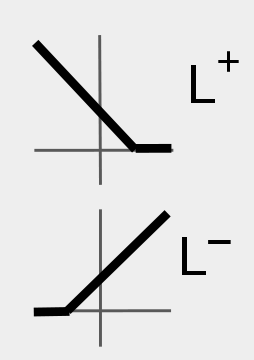
\includegraphics[width=\linewidth]{figs/cap-loss.png}}
		\end{column}
		\begin{column}{.8 \linewidth}
			\begin{itemize}
				\item Classifieurs binaires ($y_t \in \{-1,1\}$)~:
				$$ l_t = \left[1 - y_t \langle w_{t-1}, x_t \rangle \right]_+$$
			
			\end{itemize}
		\end{column}		
	\end{columns}
\end{frame}

\begin{frame}
	\frametitle{La perte "Hinge" multiclasse ($y_t \in \{1,...,K\}$)}
		\begin{exampleblock}{}
			$
			\left.
			\begin{array}{l}
			W = (w_1,..,w_K) \in \mathbb{R}^{K d}\\
			X_t^k \triangleq (\vec{0}, ...,  x_t, ..., \vec{0}) \in \mathbb{R}^{K d}
			\end{array}
			\right\}
			\text{ tels que : }
			\langle W, X^k_t\rangle = \langle w_k, x_t\rangle
			$
			
		\end{exampleblock}
		
	\begin{columns}
		\begin{column}{.2 \linewidth}
			\centerline{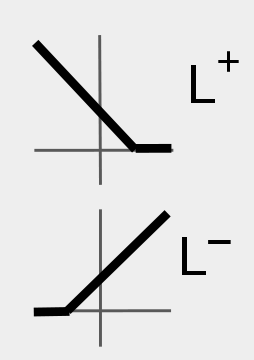
\includegraphics[width=\linewidth]{figs/cap-loss.png}}
		\end{column}
		\begin{column}{.8 \linewidth}
			\begin{itemize}
				\item Classifieurs multiclasse ~:
				\begin{itemize}
					\item Perte relative (Kessler)~:
					$$l_t =  \left[ 1 +  \langle W_{t-1}, X_t^y \rangle - \max_{k \neq y} \langle W_{t-1}, X_t^k\rangle\right]_+$$
					\item Perte absolue (One-Versus-All)~:
					$$l_t = \sum_{k=1}^K \left[1 + (1 - 2 \delta(y_t,k)) \langle W_{t-1}, X_t^k\rangle\right]_+$$
					
				\end{itemize}
			\end{itemize}
		\end{column}		
	\end{columns}
\end{frame}

\begin{frame}\frametitle{Minimisation en ligne du risque empirique}
	\begin{itemize}
		\item Approche "passive-agressive" \cite{crammer2006online}
		\item Optimisation quadratique "locale" : $\forall t$, résoudre: 
		$$W_{t} = \arg \min_W \frac{1}{2} \| W - W_{t-1}\|^2 + C \xi^2 \hbox{ s.t. } l_t \leq \xi$$
		\item Mise à jour~:
		$$W_{t} =  W_{t-1} + \frac{l_t}{2\|x_t\|^2 + \frac{1}{2C}}  (X_t^{y_t} - \max_{k \neq y} X_t^k)$$
		\item Dans le cas linéairement séparable~:
		$$\sum_{t=1}^{T} l_t^2 \leqslant 4 R^2 \parallel{U}\parallel^2$$
	\end{itemize}
\end{frame}
%\begin{frame}\frametitle{Rôle du feedback}
% \begin{itemize}
% 	\item Cas du bandit : 
% 	\begin{itemize}
% 		\item feedback quantitatif 
% 		\item $g$ est une grandeur continue
% 		\item gain, bénéfice direct de l'action
% 	\end{itemize}
% 	\item Cas des classifieurs~:
% 	\begin{itemize}
% 		\item feedback qualitatif /discret :
% 		\begin{itemize}
% 			\item consigne explicite : $y$
% 			\item consigne implicite : "bien"/"pas bien" (1 bit)
% 		\end{itemize}
% 		\item une \textit{quantité} $g$ calculée indirectement (fonction de perte)
% 	\end{itemize}
% \end{itemize}
% 
% \begin{block}{}
%Le couple feedback/fonction de perte constitue le cœur de l'algorithme d'apprentissage.
% \end{block}
% 
%\end{frame}


\begin{frame}
	\frametitle{Le feedback "1 bit" en classification}
	
	\begin{itemize}
		\item Feedback qualitatif unaire :
		\begin{itemize}
			\item réponse en "tout ou rien"
			\item clic, like, visit, follow, retweet ...
			\item caractéristique des interactions hommes machines
		\end{itemize}
		\item Dans le cadre de la classification en ligne : 
		\begin{itemize}
			\item $x_t$ est le contexte, l'étiquette $y_t$ est "cachée"
			\item La réponse proposée est $\tilde{y}_t$
			\item $f_t = {\color{red}\delta(\tilde{y}_t ,y_t)} \in \{0,1\}$
		\end{itemize}
		\item Méthodes :
		\begin{itemize}
			\item Algorithme du "Banditron" \cite{kakade2008efficient}
			\item Algorithmes de bandits contextuels
		\end{itemize}
	\end{itemize}
\end{frame}

\begin{frame}
	\frametitle{Le feedback "1 bit" dans le développement moteur}
	\centerline{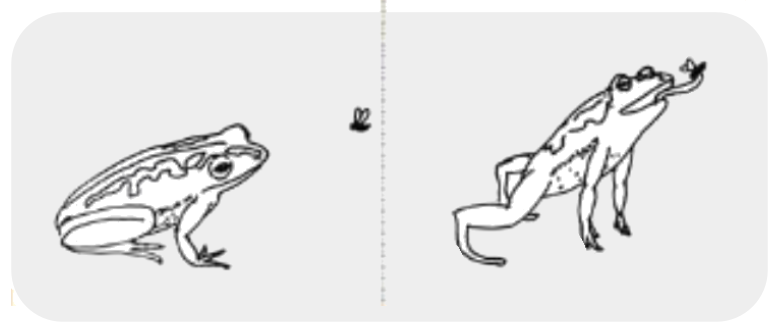
\includegraphics[width=.7\linewidth]{figs/cap-frog.png}}
	\begin{itemize}
		\item apprentissage de compétences motrices
		\item répertoire d'actions
		\item gratification en "tout ou rien"
	\end{itemize}
\end{frame}


\begin{frame}
	\frametitle{Le Banditron \cite{kakade2008efficient}}

	\begin{block}{}
		$\forall t \in 1,...,T :$
		\begin{align*}
		&\text{1. Lire } 
		&& x_t 
		\\
		&\text{2. Choisir :} 
		&& \hat{y}_t = \underset{k \in\{1,..,K\}}{\text{argmax}}  \langle W_{t-1}, X_t^k \rangle 
		\\
		& %\text{3. Décision }\tilde{y}_t\text{ : } 
		&& \tilde{y}_t \sim (1-\varepsilon) \delta(k,\hat{y}_t) + \frac{\varepsilon}{K} 
		\\	
		&\text{3. Lire } 
		&& {\color{red} f_t = \delta(\tilde{y}_t ,y_t)}  
		\\
		&\text{4. Mettre à jour :} 
		&& W_t = W_{t-1} + \frac{{\color{red}f_t}\cdot X_t^{\tilde{y}_t}}{P(\tilde{Y}_t=\tilde{y}_t)} - X_t^{\hat{y}_t} 
		\end{align*}
	\end{block}

\end{frame}

\begin{frame}\frametitle{Intervalles de confiance}
	\begin{itemize}
		\item Bandits contextuels
		\item Choix basé sur :
		\begin{itemize}
			\item Les intervalles de confiance (UCB)\cite{lai1985asymptotically}
			\item Le Perceptron d'ordre 2 \cite{cesa2005second}
		\item Exemples :
		\begin{itemize}
		 \item\cite{li2010contextual}
		 \item\cite{hazan2011newtron}
		 \item\cite{crammer2013multiclass}
		 \item\cite{ngo2013upper}
		 \end{itemize}
		\end{itemize} 
		\item Regret $O(\sqrt{T})$ dans le cas stationnaire.
		\item La mise à jour repose sur une estimateur de 
		$\mathbb{E}\left[ {X_t^{\hat{y}_t}}^\top \cdot X_t^{\hat{y}_t}\right]$:
		\begin{itemize}
			\item Coût $O(d^2)$ en espace
			\item Non sparse
		\end{itemize}
	\end{itemize}
	
\end{frame}
	


\begin{frame}\frametitle{Perte Hinge : réduction au cas du "bandit"}
	\begin{columns}
		\begin{column}{.2 \linewidth}
			\centerline{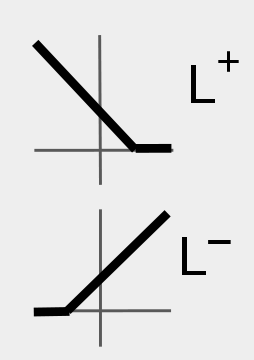
\includegraphics[width=\linewidth]{figs/cap-loss.png}}
		\end{column}
		\begin{column}{.8 \linewidth}
			\begin{itemize}
				\item Réduction (échantillon) de la perte OVA~: 
				$$l_t =  \left[1 + (1 - 2 {\color{red}\delta(y_t,\tilde{y}_t)}) \langle W_{t-1}, X_t^{\tilde{y}_t}\rangle\right]_+$$

				\item Minimisation en ligne du risque empirique~:
				$$W_{t} =  W_{t-1} + \frac{l_t}{\|x_t\|^2 + \frac{1}{2C}}  (2 {\color{red}\delta(y_t,\tilde{y}_t)} - 1) X_t^{\tilde{y}_t}$$		
				\item Agressivité / conservatisme ($C \rightarrow \infty$)~:
				\begin{itemize}
					\item apprentissage en un coup
					\item sensibilité aux erreurs de label
				\end{itemize}	
			\end{itemize}
		\end{column}
	\end{columns}
\end{frame}

\begin{frame}
	\frametitle{Le Bandit "passif-agressif" (BPA)}
%	\begin{exampleblock}{}
%		$
%		\left.
%		\begin{array}{l}
%		W = (w_1,..,w_K) \in \mathbb{R}^{K d}\\
%		X_t^k \triangleq (\vec{0}, ...,  x_t, ..., \vec{0}) \in \mathbb{R}^{K d}
%		\end{array}
%		\right\}
%		\text{ tels que : }
%		\langle W, X^k_t\rangle = \langle w_k, x_t\rangle
%		$
%		
%	\end{exampleblock}
	
	\begin{block}{}
		$\forall t \in 1,...,T :$
		\begin{align*}
		&\text{1. Lire } 
		&& x_t 
		\\
		&\text{2. Choisir :} 
		&& \hat{y}_t = \underset{k \in\{1,..,K\}}{\text{argmax}}  \langle W_{t-1}, X_t^k \rangle 
		\\
		& %\text{3. Décision }\tilde{y}_t\text{ : } 
		&& \tilde{y}_t \sim (1-\varepsilon) \delta(k,\hat{y}_t) + \frac{\varepsilon}{K} 
		\\	
		&\text{3. Lire } 
		&& {\color{red} f_t = \delta(\tilde{y}_t ,y_t)}  
		\\
		&\text{4. Mettre à jour :} 
		&& W_t = W_{t-1} + \frac{l_t}{\|x_t\|^2 + \frac{1}{2C}} (2{\color{red}f_t}-1)\cdot X_t^{\tilde{y}_t}
		\end{align*}
	\end{block}
	
\end{frame}

\begin{frame}{Cas linéairement séparable}
	\begin{theorem}
		\label{theo:BPAT1}
		Soit $(x_1,y_1),...,(x_T,y_T)$ une séquence d'exemples linéairement séparables où $x_t \in \mathbb{R}^d$, $y_t\in \{1,...,K\}$ et $\parallel x_t \parallel\leqslant R$ pour tout $t$, soit $\tilde{y}_1,...,\tilde{y}_T$ une séquence de réponses, et soit $U \in \mathbb{R}^{K\times d}$ tel que $ \forall t, l^*_t=0$. Alors, en supposant $C \rightarrow \infty$, la perte au carré cumulée du BPA est bornée par:
		\begin{equation*}
		\sum_{t=1}^{T} l_t^2 \leqslant R^2\cdot \parallel{U}\parallel^2
		\end{equation*}
	\end{theorem}
	
	\begin{alertblock}{Attention!!}
		La somme des pertes au carré n'est pas ici un majorant de la somme des erreurs de prédiction.
	\end{alertblock}
\end{frame}

\begin{frame}{Conditions supplémentaires}
	On peut montrer que, pour une politique de choix "avide"~:
	\begin{itemize}
		\item Si $\exists t^*$ tel que $\forall t \geq t^*, l_t =0$
		\item Si les vecteurs d'observation  de la classe $k$ sont issus d'un ensemble convexe $\mathcal{C}_k \subset \mathbb{R}^d$
		\item Si $\exists t \geq t^*$ tel que $\tilde{y}_t = y_t = k$
	\end{itemize}
	alors \textit{tous} les exemplaires de la classe $k$ sont correctement classifiés par $W_t$ pour $t \geq t^*$.
	
	Cette situation peut en outre être garantie presque sûrement si: 
	$$\tilde{y}_t \sim (1-\varepsilon) \delta(k,\hat{y}_t) + \frac{\varepsilon}{K} $$
\end{frame}

\begin{frame}{Cas stationnaire}
	\begin{footnotesize}
	\begin{theorem}
		Soit $(x_1,y_1),...,(x_T,y_T)$ une séquence d'exemples linéairement séparables où $x_t \in \mathbb{R}^d$, $y_t\in \{1,...,K\}$ et $\parallel x_t \parallel\leqslant R$ pour tout $t$, soit $\tilde{y}_1,...,\tilde{y}_T$ une séquence de réponses, et soit $U \in \mathbb{R}^{K\times d}$ un classifieur quelconque. Alors, en supposant $C \rightarrow \infty$, la perte au carré cumulée du BPA est bornée par:
		\begin{equation*}
	\sum_{t=1}^{T}l_t^2 \leqslant \left(R\parallel{U}\parallel+2 \sqrt{\sum_{t=1}^{T}(l_t^{\ast})^2}\right)^2 
		\end{equation*}
	\end{theorem}

	\begin{alertblock}{}
		\begin{itemize}
			\item Pour les temps longs, une perte moyenne au pire double de la perte optimale
			\item Nécessite un $C$ fini pour atteindre un regret en $O(\sqrt{T})$
		\end{itemize}
	\end{alertblock}
	\end{footnotesize}
\end{frame}

\begin{frame}{Extension à l'approche noyaux}

	\begin{itemize}
		\item Soit $\mathcal{K}(.,.)$ une application de $ \mathbb{R}^d \times \mathbb{R}^d$ dans $ \mathbb{R}^+$ ayant la propriété de reproduction,
		\item soit $\mathcal{H}$ le RKHS correspondant,
	\item Soit $\mathcal{K}(x,.)$ la projection de l'exemplaire $x$ dans $\mathcal{H}$. 
	\item Alors : 
	%$$\forall w \in \mathcal{H}, \langle w,\mathcal{K}(x,.)\rangle_\mathcal{H} = w(x) $$
	\end{itemize}
	\begin{footnotesize}
	\begin{exampleblock}{}
		$
		\left.
		\begin{array}{l}
		W = (w_1,..,w_K) \in \mathcal{H}^K\\
		X_t^k \triangleq (0(.), ..., \mathcal{K}(x_t,.), ..., 0(.)) \in \mathcal{H}^{K}
		\end{array}
		\right\}
		\langle W,X^k\rangle \triangleq \langle w_k,\mathcal{K}(x,.)\rangle_\mathcal{H} = w_k(x)
		$
		
	\end{exampleblock}
	\end{footnotesize}	
\end{frame}

\begin{frame}{Expérimentations}
	\begin{table}[h]
		\caption{Five datasets considered, with $n$ the number of instances, $d$ the vectors dimension and $K$ the number of labels.}
		\label{table:mce}
		\begin{center}
			\begin{tabular}{l l l l}
				{\bf Dataset}  & {\bf $n$} & {\bf $d$} & {\bf $K$}\\
				\hline
				SynSep & $10^5$ 	& 400 	& 9 \\
				
				SynNonSep & $10^5$ & 400 	& 9 \\
				
				RCV1-v2  & $10^5$ 	& 47236 	& 53 \\
				
				Segment & 2310	& 19	& 7	\\
				
				Pendigits 	& 7494	& 16	& 10	\\
			\end{tabular}
		\end{center}
	\end{table}
\end{frame}

\begin{frame}{Expérimentations}
	\begin{small}
	\begin{table}[h]
		\caption{Parameters setting for different algorithms and different datasets. }
		% {\bf P} stands for Perceptron, {\bf PA} for Passive Agressive, {\bf B} for Banditron, {\bf C} for Confidit, {\bf BPA} for the one-Bit feedback Passive Aggressive (algorithm 1), {\bf K-B} for the kernel Banditron, {\bf K-BPA}  for the kernel  realization of BPA (algorithm 1) and {\bf K-SGD} for the kernel  realization of SGD (algorithm 2).}
		%\label{table:bpa}
		%\begin{center}
		
		%		\begin{tabular}{llllll}
		%			
		%			\hline
		%			{\bf }  & {\bf P} & {\bf PA } & {\bf B}& {\bf C} & {\bf BPA}\\
		%			\hline
		%			SS & $\varnothing$ & $C=0$ & $\varepsilon = 0.014$ &$\eta = 10^3$ & $\varepsilon = 0.4$\\
		%			&&&&& $C = \infty$\\
		%			
		%			SN & $\varnothing$ & $C=10^{-2}$ & $\varepsilon =0.65$ & $\eta = 10^3$& $\varepsilon = 0.8$\\
		%			&&&&& $C = 10^{-2}$\\			
		%			R & $\varnothing$ & $C=10^{-2}$ & $\varepsilon =0.4$ & $\eta = 10^2$ & $\varepsilon = 0.2$\\
		%			&&&&& $C = 10^{-2}$\\
		%			\hline
		%			&{\bf KB} & {\bf BPA} & {\bf KBPA} &{\bf KSGD}\\
		%			\hline
		%			P & $\sigma = 1$ & $C = 10^{-2}$ &$\sigma = 1$&$\sigma = 1$\\
		%			&&$\varepsilon = 0.2$& $C = 1$ & $H = 500$\\
		%			&&& $\varepsilon = 0.2$ &\\
		%			S & $\sigma = 10$ & $C = 10^{-2}$ & $\sigma = 10$&$\sigma = 10$\\
		%			&&$\varepsilon = 0.2$& $C = 1$& $H = 200$\\
		%			&&& $\varepsilon = 0.2$ &
		%			%LR(26 letters) & null &  $C=0.1$ & $\varepsilon = 0.2$& $\eta=10^2$ & $\varepsilon = 0.8,C= 1$ \\
		%			
		%			%LR(10 numbers) & null & $C=0.1$ & $\varepsilon= 0.4$& $\eta = 10$ & $\varepsilon = 0.6,C=1$\\
		%			
		%		\end{tabular}
		%\hspace{-.8cm}
		\begin{center}
			\begin{tabular}{llllll}
				
				\hline
				{\bf Dataset}  & {\bf P} & {\bf PA } & {\bf B}& {\bf C} & {\bf BPA}\\
				\hline
				Synsep & $\varnothing$ & $C\rightarrow\infty$ & $\varepsilon = 0.014$ &$\eta = 10^3$ & $\varepsilon = 0.4$\\
				&&&&& $C \rightarrow \infty$\\
				
				SynNonSep & $\varnothing$ & $C=10^{-2}$ & $\varepsilon =0.65$ & $\eta = 10^3$& $\varepsilon = 0.8$\\
				&&&&& $C = 10^{-2}$\\			
				RCV1-v2 & $\varnothing$ & $C=10^{-2}$ & $\varepsilon =0.4$ & $\eta = 10^2$ & $\varepsilon = 0.2$\\
				&&&&& $C = 10^{-2}$\\
				\hline
				&{\bf K-B} & {\bf BPA} & {\bf K-BPA} &{\bf K-SGD}\\
				\hline
				Segment & $\sigma = 1$ & $\varepsilon = 0.3$ & $\sigma = 1$ &$\sigma = 1$\\
				&$\varepsilon =0.1$&&$\varepsilon = 0.3$ & $H = 200$\\
				Pendigits & $\sigma = 10$ & $\varepsilon = 0.3$ &$\sigma = 10$&$\sigma = 10$\\
				&$\varepsilon =0.1$&& $\varepsilon = 0.3$ & $H = 500$\\
				
				%LR(26 letters) & null &  $C=0.1$ & $\varepsilon = 0.2$& $\eta=10^2$ & $\varepsilon = 0.8,C= 1$ \\
				
				%LR(10 numbers) & null & $C=0.1$ & $\varepsilon= 0.4$& $\eta = 10$ & $\varepsilon = 0.6,C=1$\\	
			\end{tabular}	
		\end{center}
	\end{table}
	\end{small}
\end{frame}

\begin{frame}{Taux d'exploration}
	%\begin{figure}[htp]
		%\centerline{\bf (a)}
		\begin{columns}
			\begin{column}{.5\linewidth}
				\centerline{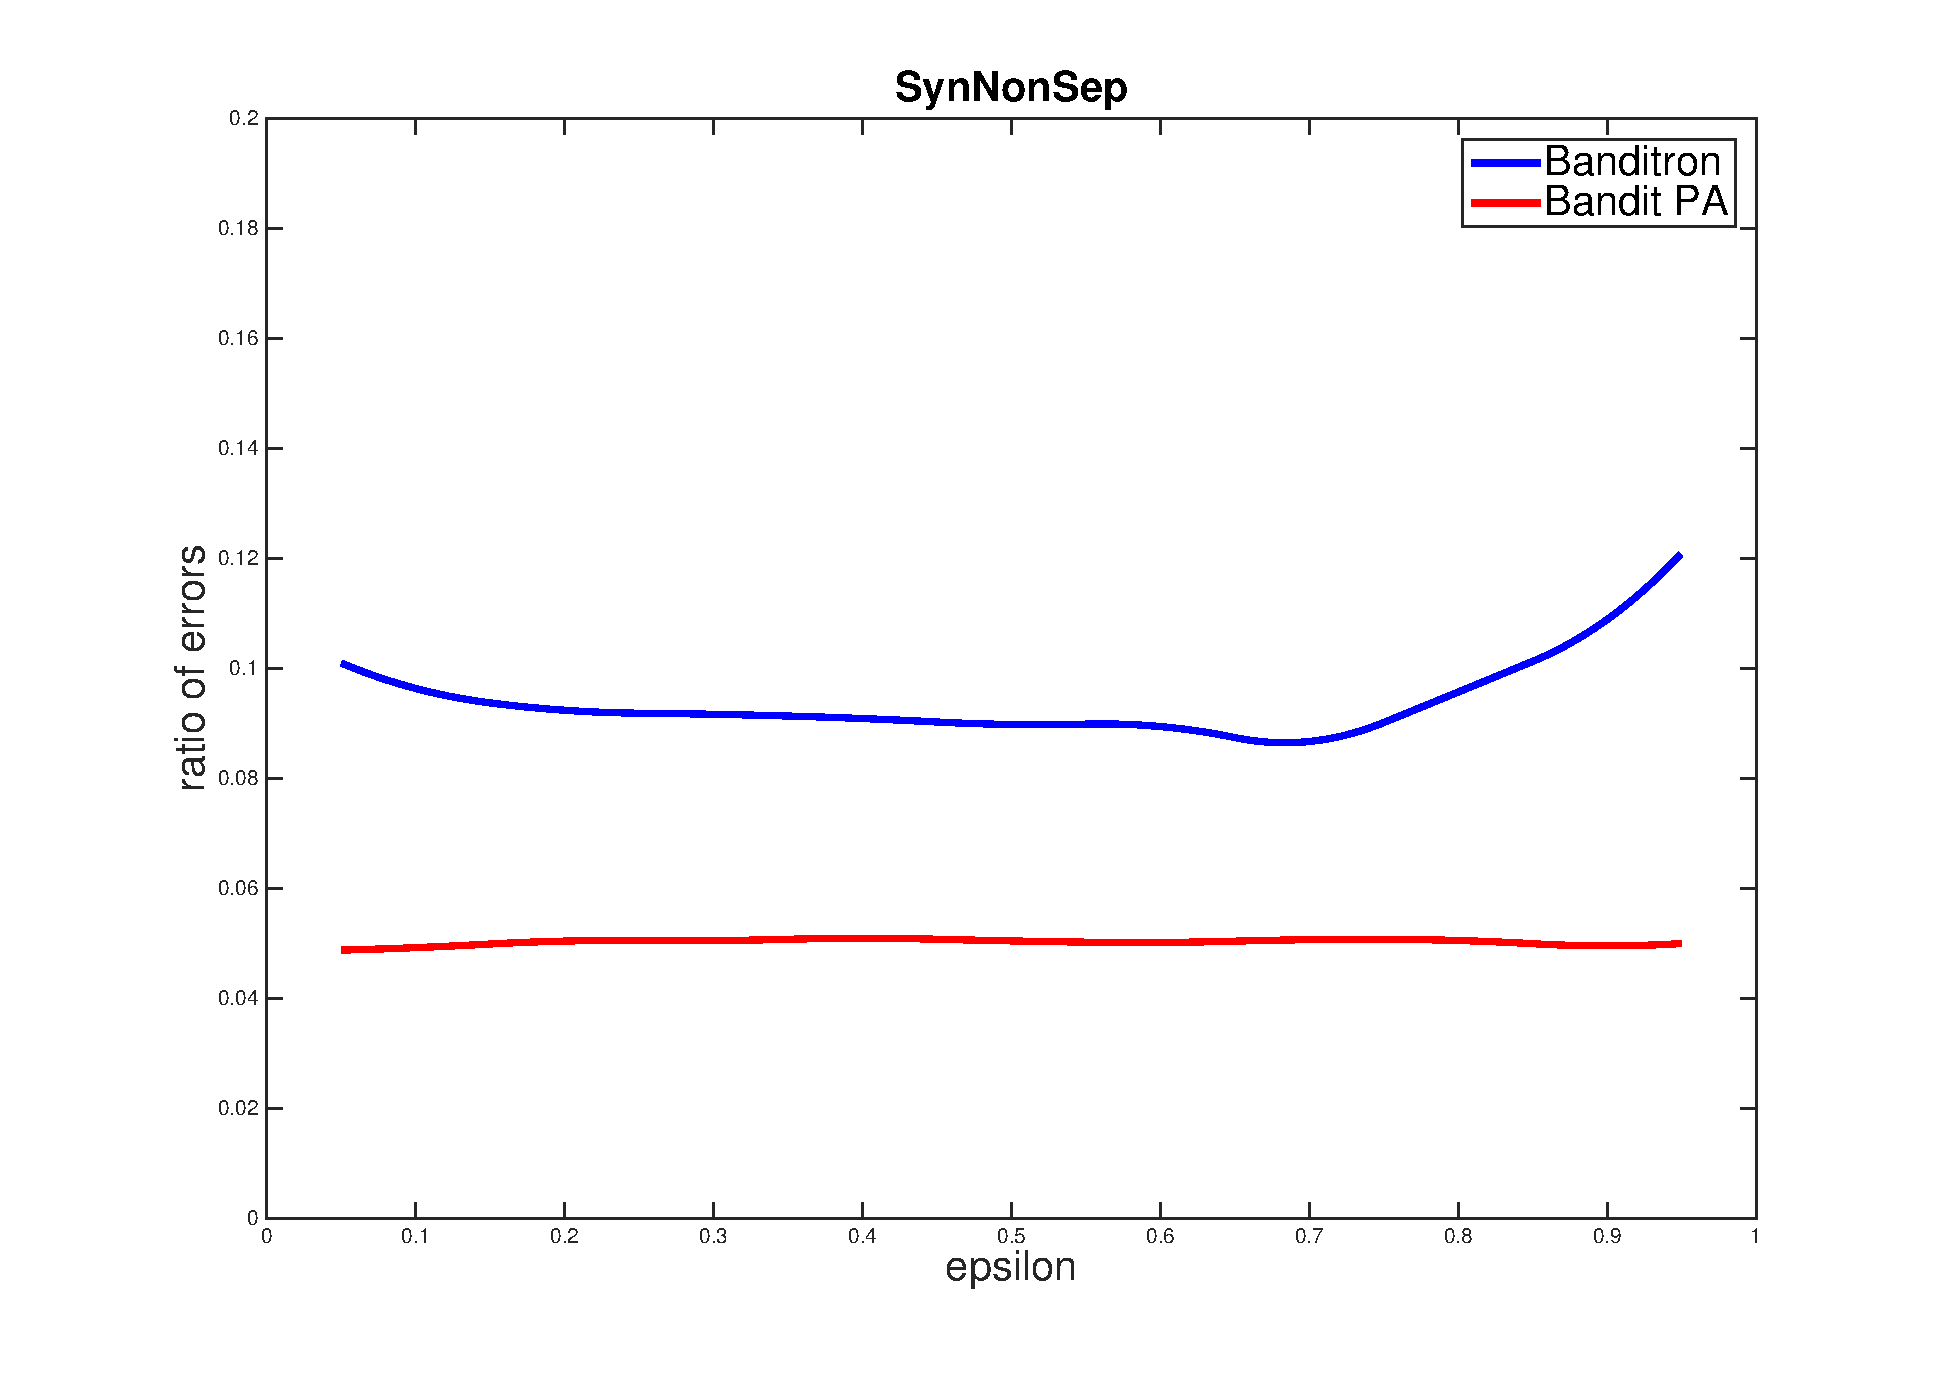
\includegraphics[width=\linewidth]{figs/SynNonSep_gamma.eps}}
				%\centerline{\bf (b)}
				\centerline{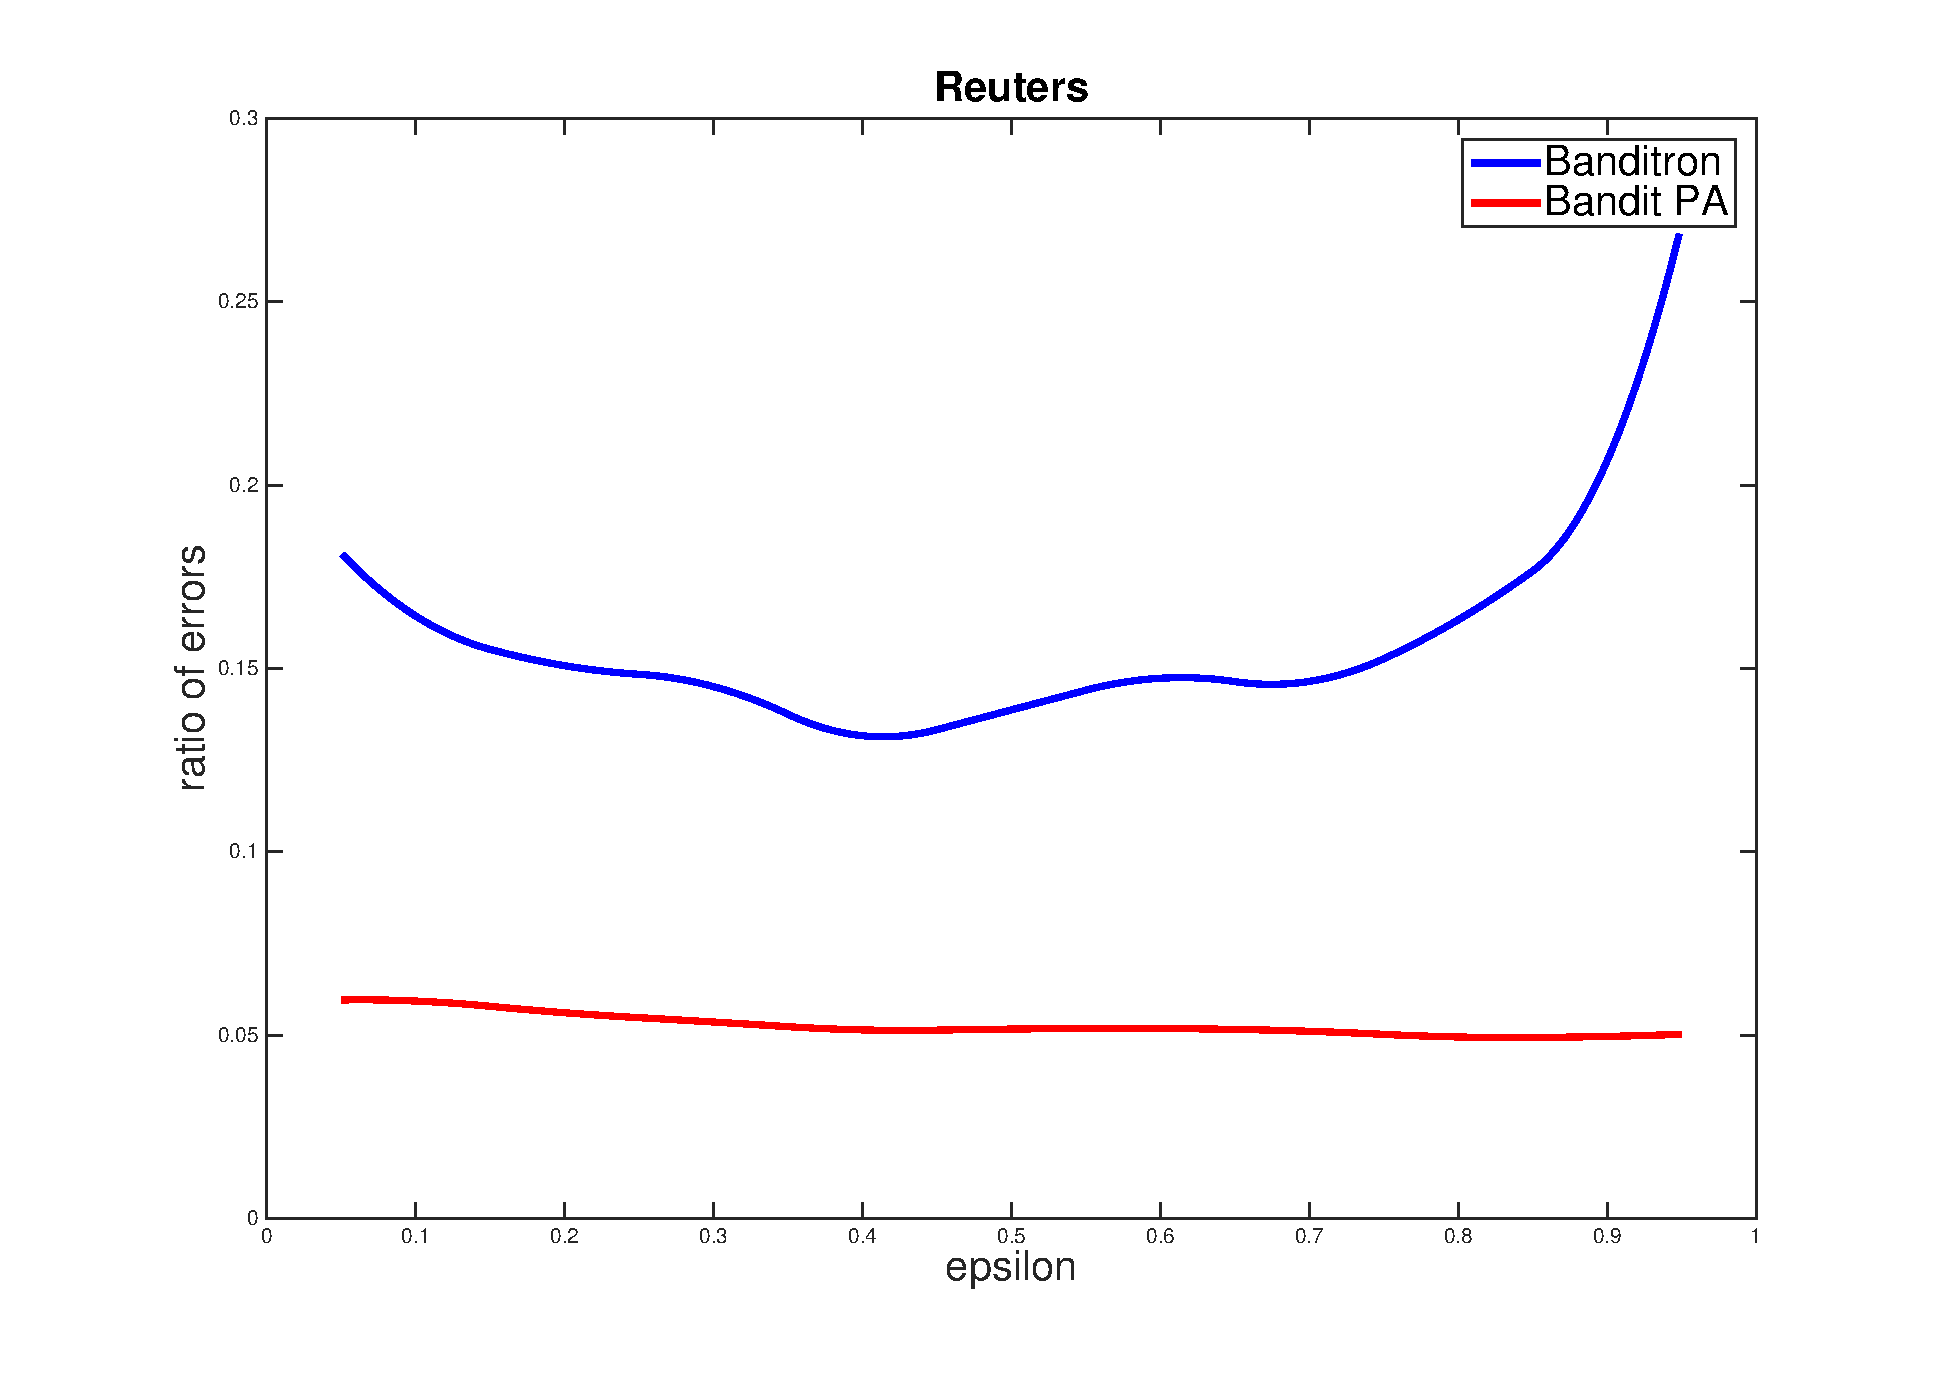
\includegraphics[width=\linewidth]{figs/Reuters_gamma.eps}}
			\end{column}
			\begin{column}{.5\linewidth}
				\begin{itemize}
					\item Taux d'erreur final en fonction du taux d'exploration $\varepsilon$
					\item SynNonSep (top) and Reuters (bottom) datasets.
				\end{itemize}
			\end{column}	
		\end{columns}
		
		%\end{figure}
		
		%\begin{figure}[ht!]
		
		%\caption{Taux d'erreur moyen du Banditron et du BPA en fonction du taux d'exploration $\varepsilon$ }
		%\label{pic:BPARCVerr}
	%\end{figure}
\end{frame}

\begin{frame}{Erreur cumulée}
			\begin{columns}[t]
				\begin{column}{.5\linewidth}
	\centerline{
		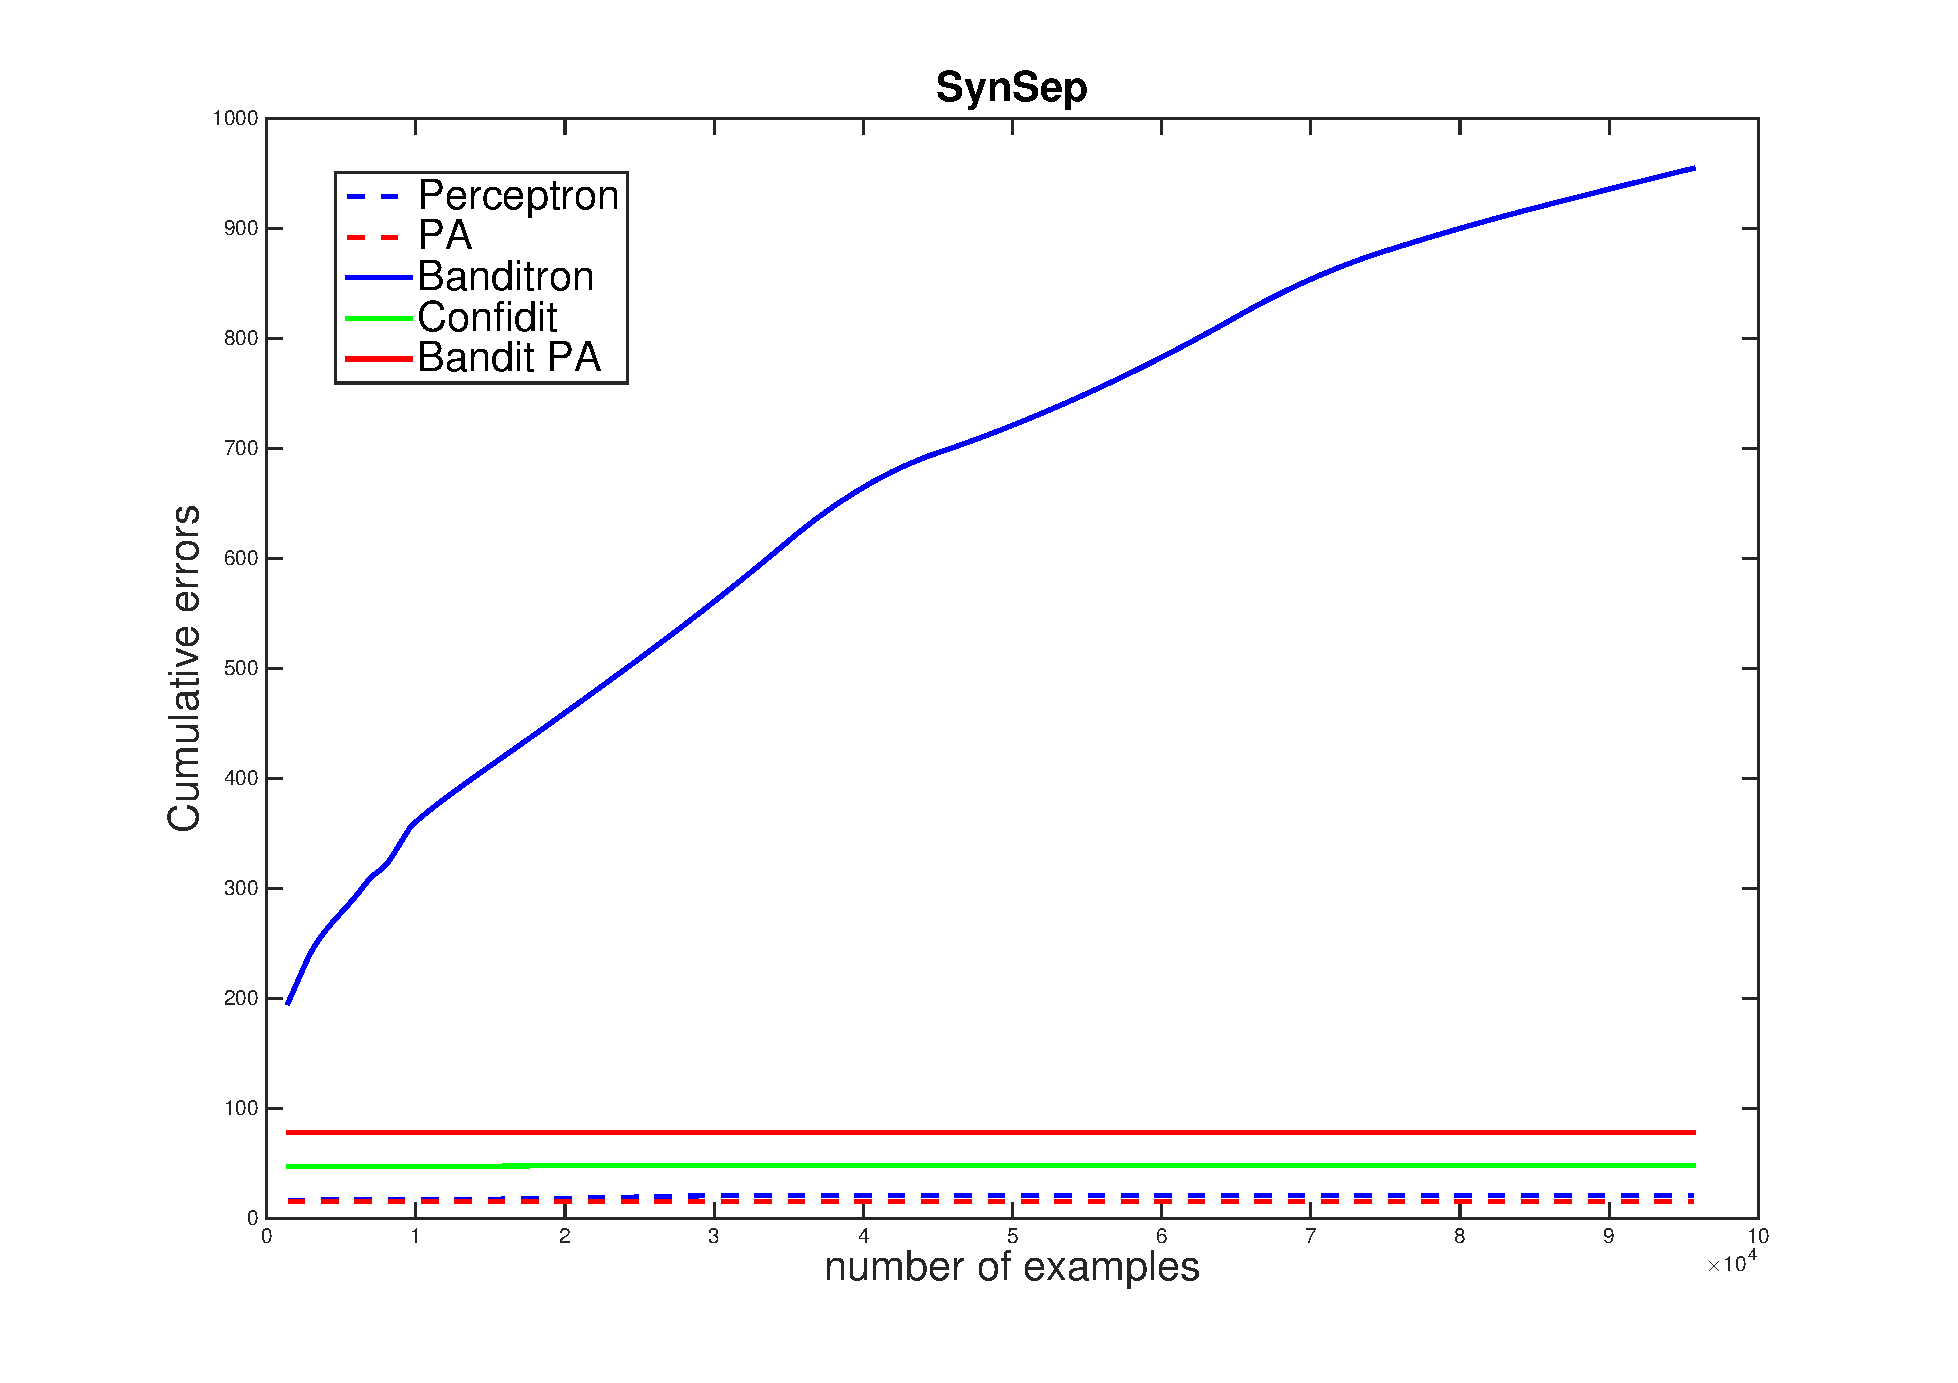
\includegraphics[width=\linewidth]{figs/SynSep.eps}
	}
	
	\centerline{
		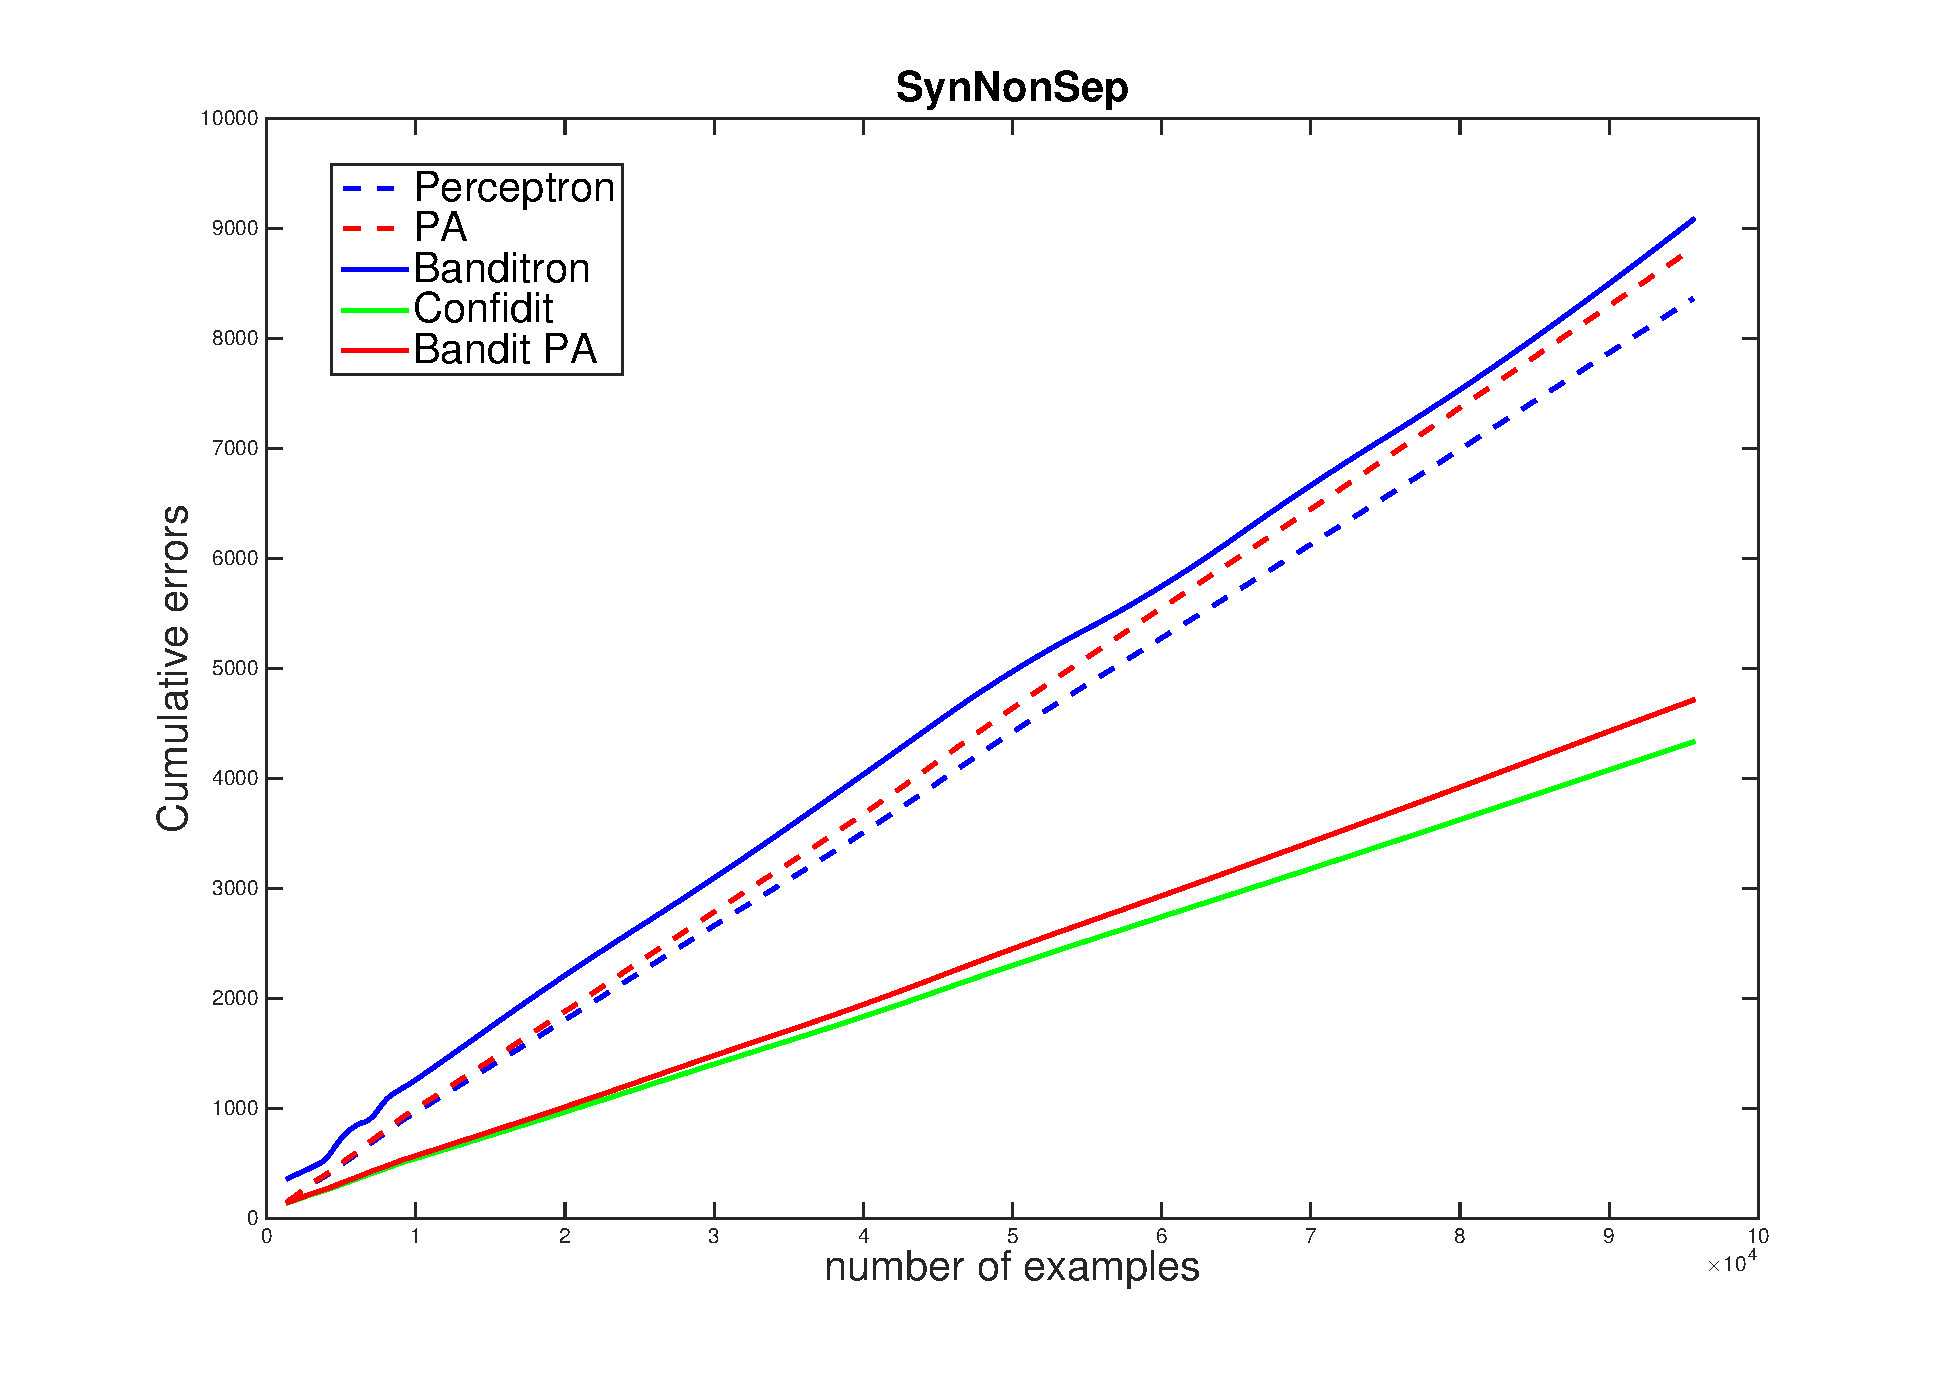
\includegraphics[width=\linewidth]{figs/SynNonSep.eps}
	}
				\end{column}
				\begin{column}{.5\linewidth}
		\centerline{
			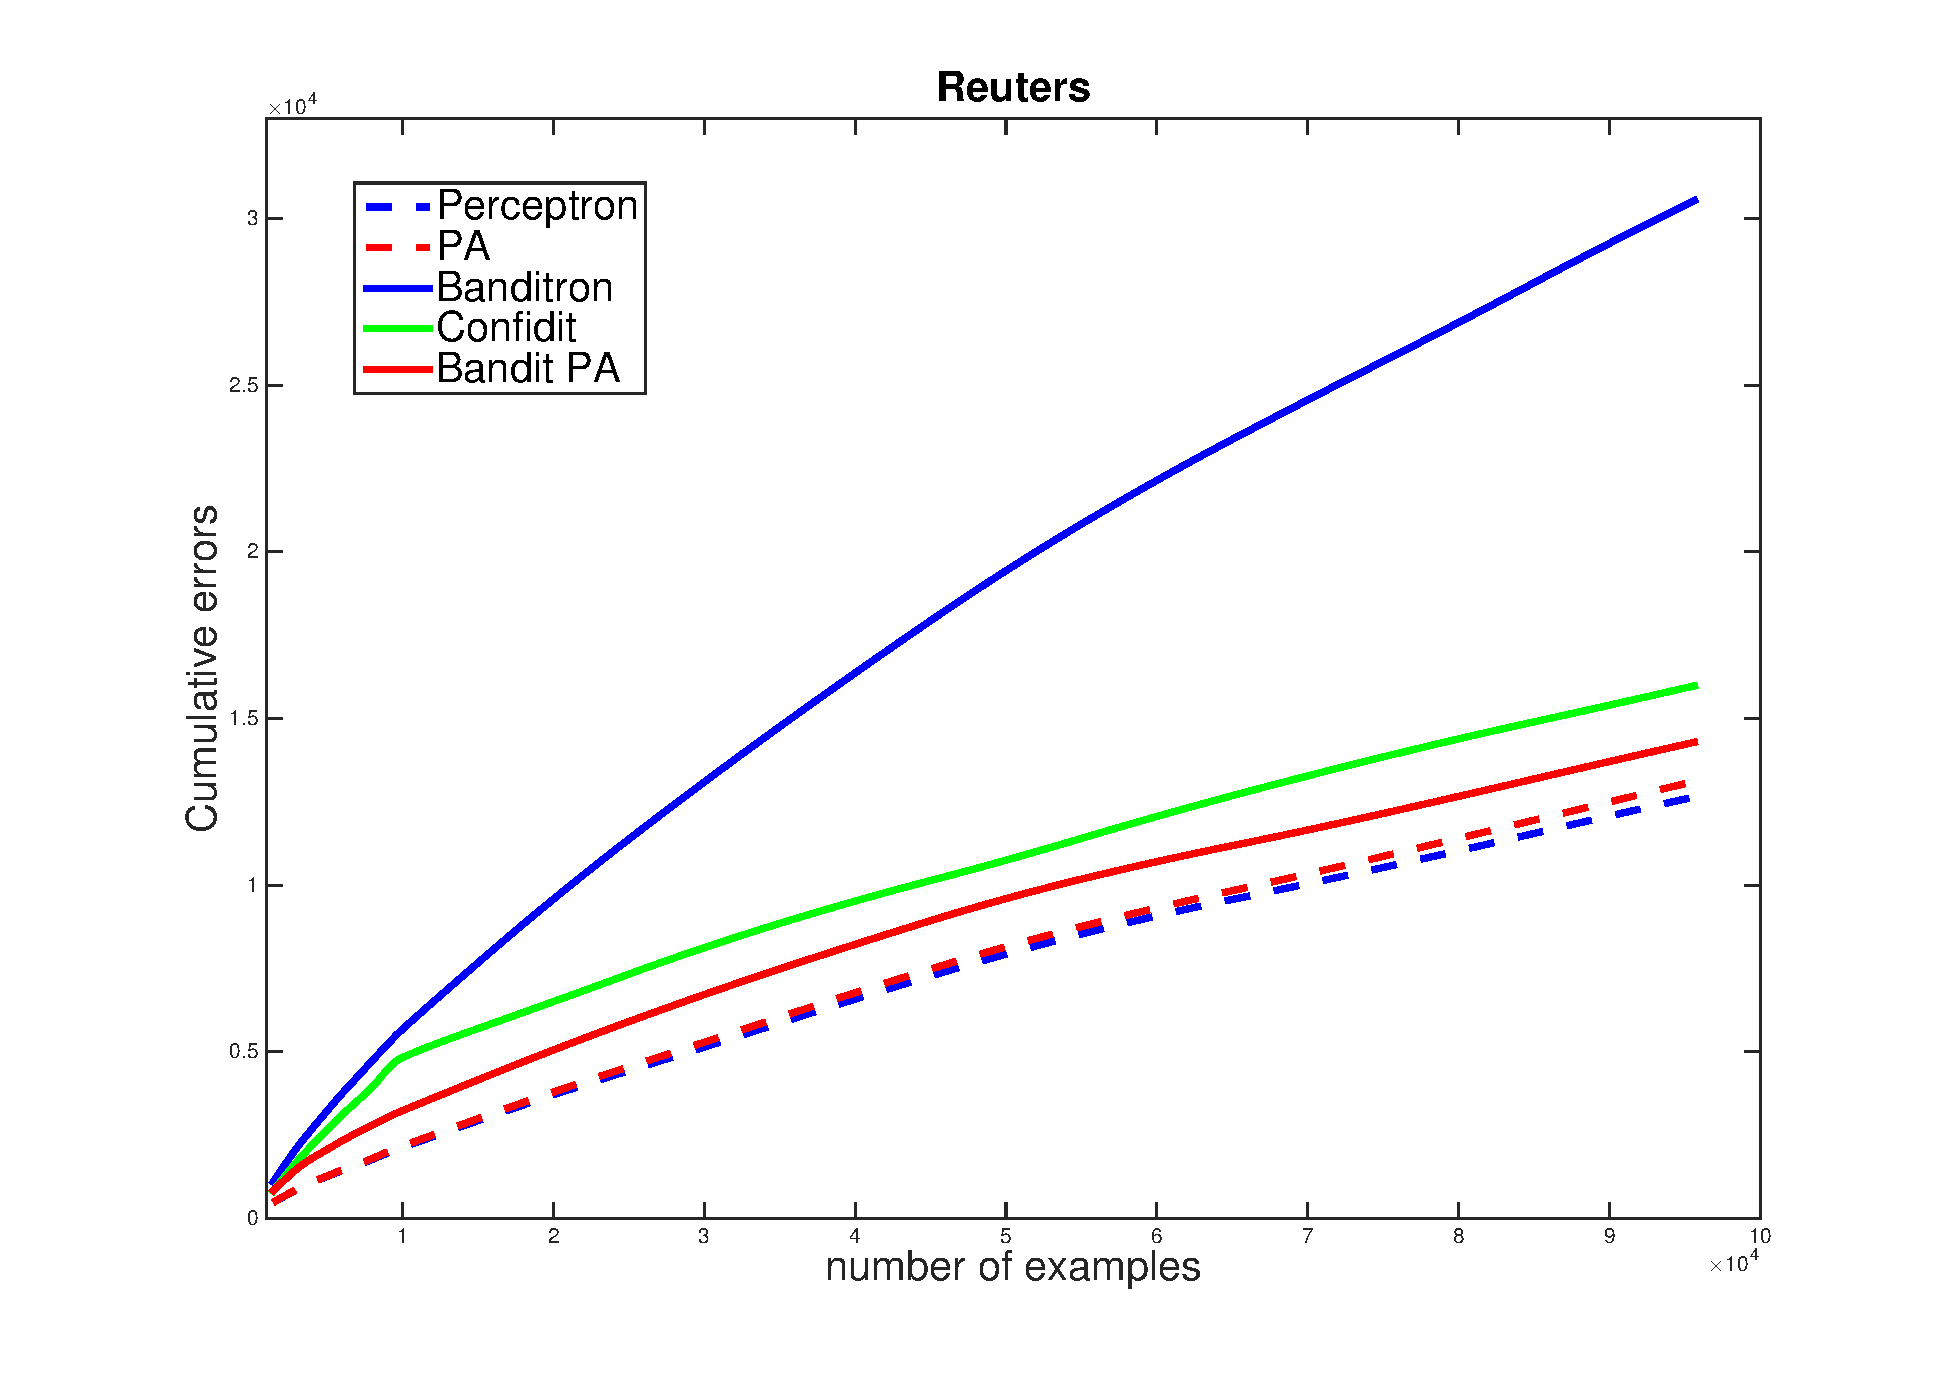
\includegraphics[width=\linewidth]{figs/RCV1_v2_53class.eps}}
		\begin{footnotesize}
		\begin{itemize}
			\item Perceptron, PA, Banditron, Confidit et BPA
			\item SynSep (9 classes), SynNonSep (9 classes) et Reuters (53 classes)
		\end{itemize}
		\end{footnotesize}

		\end{column}	
			\end{columns}
\end{frame}

\begin{frame}{Fonctions noyaux}
	\begin{columns}[t]
		\begin{column}{.45\linewidth}
\centerline{
	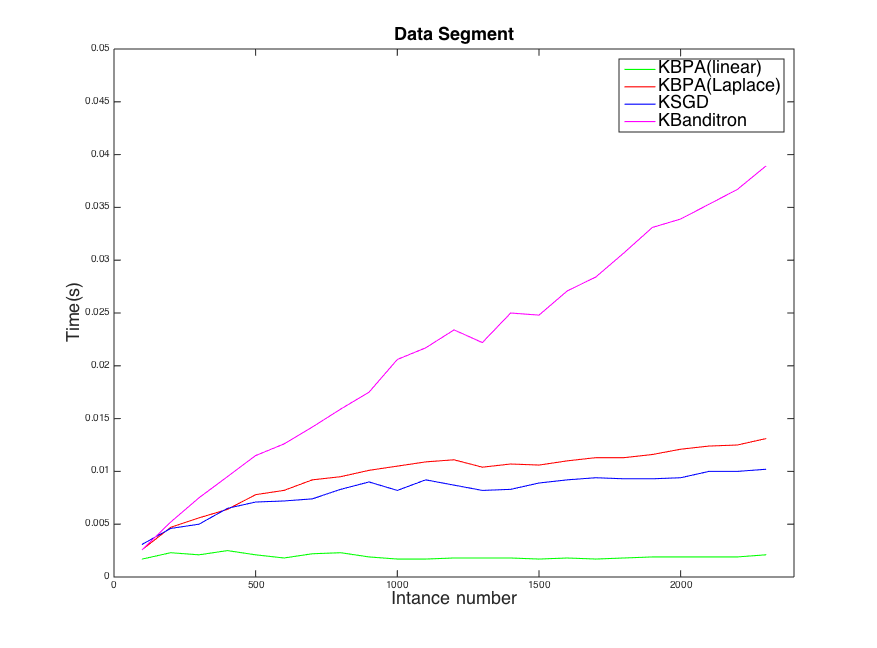
\includegraphics[width=\linewidth]{figs/Segment_kernel_T.png}}
\centerline{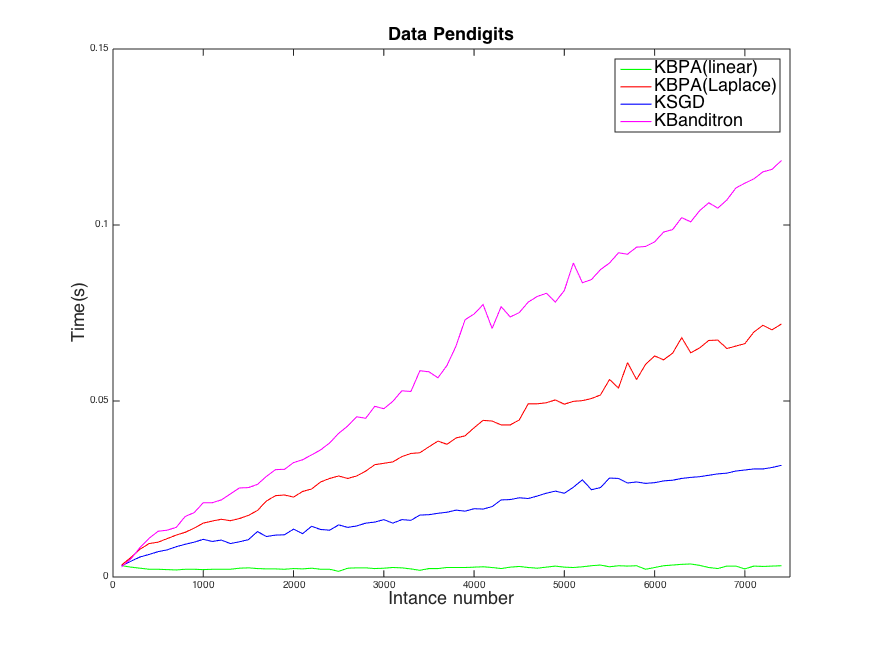
\includegraphics[width=\linewidth]{figs/Pendigits_kernel_T.png}}			
		\end{column}
		\begin{column}{.45\linewidth}
	\centerline{
		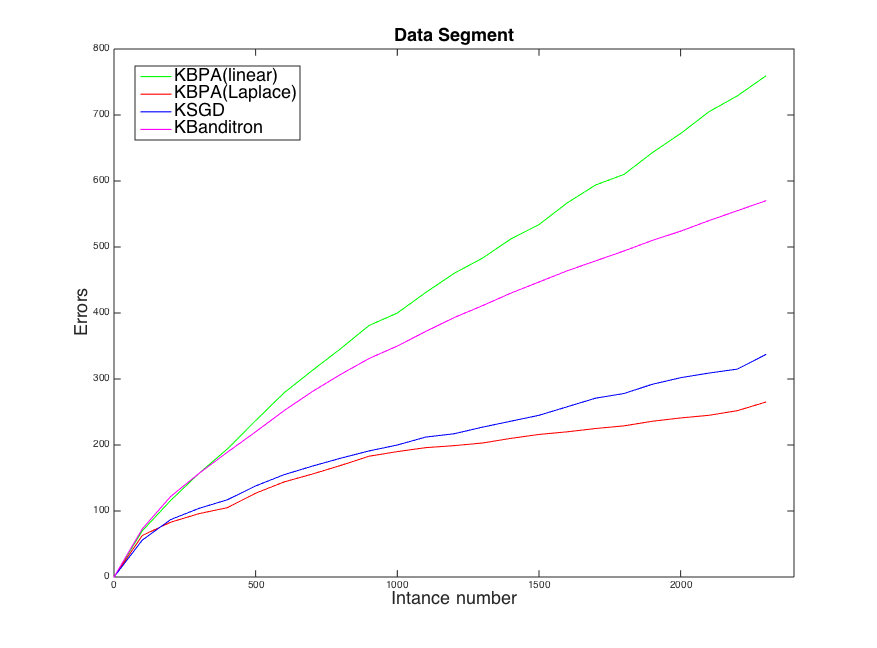
\includegraphics[width=\linewidth]{figs/Segment_kernel_CM.png}}
	\centerline{
		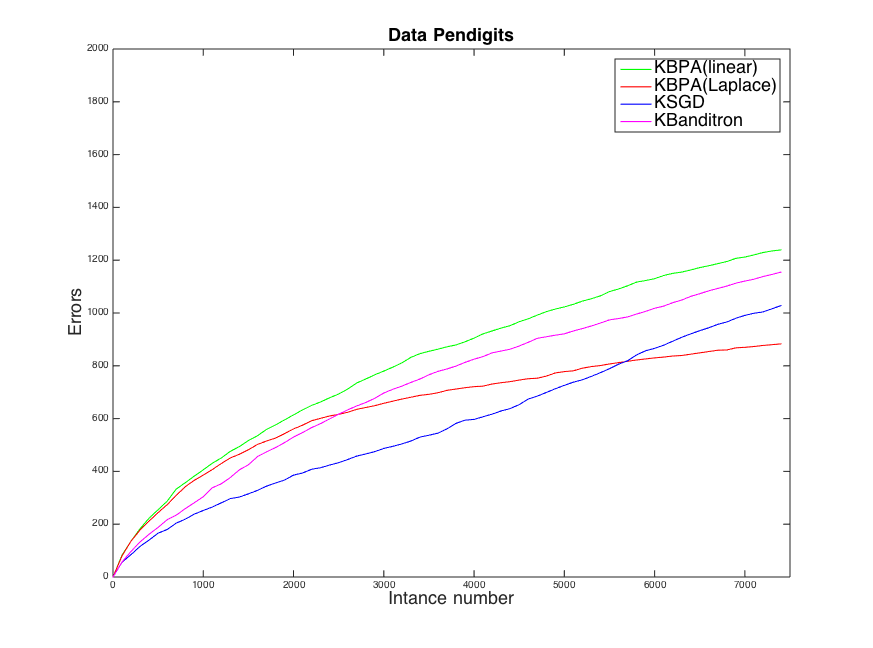
\includegraphics[width=\linewidth]{figs/Pendigits_kernel_CM.png}}
		\end{column}	
	\end{columns}
\end{frame}

\begin{frame}{Conclusion}
	\begin{itemize}
		\item Passive Aggressive Bandit feedback~:
		\begin{itemize}
			\item Une information d'étiquetage limitée (1-bit)
			\item Un apprentissage actif (par sondage) sur l'espace des labels 
			\item Principe d'aversion à l'erreur (OVA)
			\item Minimisation en ligne du risque empirique (optimisation quadratique locale sous contraintes)
		\end{itemize} 
		\item La perte au carré est bornée dans le cas linéairement séparable
		\item Des conditions raisonnables de redondance des données assurent un classification correcte en environnement stationnaire
		\item Parcimonie
		\item Facile à mettre en œuvre
		\item Passage à l'échelle OK (coût linéaire en espace)
	\end{itemize}
\end{frame}

\begin{frame}{Remarques}
	\begin{alertblock}{Un résultat contre intuitif}
		\begin{itemize}
		\item Agressivité / one shot / parcimonie:
		\begin{itemize}
			\item En principe : réponse exagérée au bruit de label
			\item Mise à jour sous-optimale dans les environnements stochastiques (bandit)
		\end{itemize}  
		\item L'aggressivité de l'algorithme nécessite d'être atténuée par un paramètre de "raideur" $C$
			\begin{itemize}
				\item $\rightarrow$ Regret en $O(\sqrt{T})$ dans le cas stationnaire
				\item Bonne résistance au bruit de label
			\end{itemize}
		\item Sous-échantillonnage d'un problème sur-contraint
		\end{itemize}
	\end{alertblock}
	
	\begin{exampleblock}{Mise en oeuvre pratique}
		\begin{itemize}
		\item Validation croisée pour $C$ (valeur spécifique au problème)
		\item Faire décroître $\varepsilon$ au cours du temps.
		\end{itemize}
	\end{exampleblock}
		
\end{frame}

\begin{frame}{Questions ouvertes}
	\begin{itemize}
		\item Vers un apprentissage moins agressif? Basé sur un modèle?
		\begin{itemize}
			\item Moindre parcimonie
			\item Risque de sensibilité au déséquilibre de classe (OVA)
			\item Borne d'erreur plus difficile à prouver
		\end{itemize}  
		\item Extension aux environnements de jeux/avec adversaire :
		\begin{itemize}
			\item Extension au cas non-stationnaires \cite{kivinen2004online} 
			\item Coups multiples, récompense différée (temporal credit assignment) \cite{sutton1998reinforcement}
			\item IHM, personal computing, compagnons,..
		\end{itemize}  		
		\item Continuum entre l'apprentissage supervisé et l'apprentissage par renforcement?
	\end{itemize}
	\vspace{-.7cm}
	\begin{columns}[t]
		\begin{column}{.01\linewidth}
		\end{column}
		\begin{column}{.4\linewidth}
			\begin{small}
			\begin{itemize}
				\item Cas des labels multiples
				\item Un "crédit" d'information entre 1 et $K$?
			\end{itemize} 
			\end{small}
		\end{column}
		\begin{column}{.4\linewidth}
			\begin{block}{}
				\centerline{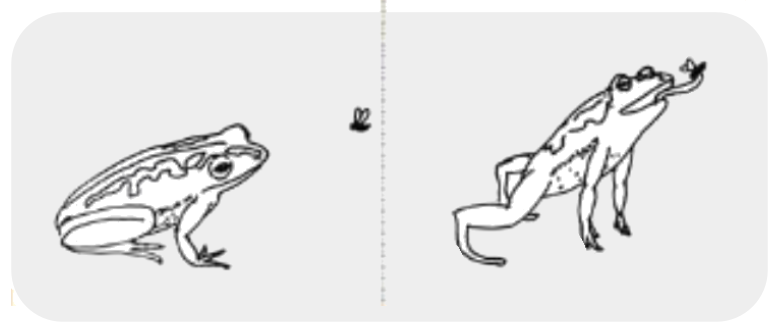
\includegraphics[width=\linewidth]{figs/cap-frog.png}}
			\end{block}
		\end{column}
	\end{columns}
	

		
\end{frame}

\bibliographystyle{apalike}
\bibliography{cap2016}
\end{document}